% !TeX encoding = UTF-8
% !TeX program = xelatex
% !TeX spellcheck = en_US

\documentclass{cjc}

\usepackage{booktabs}
\usepackage{algorithm}
\usepackage{algorithmic}
\usepackage{siunitx}
\usepackage{silence}
\hbadness=10000 \vbadness=10000 
\WarningFilter{Fancyhdr}{\headheight is too small}

\classsetup{
  % 配置里面不要出现空行
  title        = {代码克隆检测},
  title*       = {Code Reuse Detection},
%   authors      = {
%     author1 = {
%       name         = {作者名},
%       name*        = {NAME Name-Name},
%       affiliations = {aff1},
%       biography    = {性别,xxxx年生,学位(或目前学历),职称,是/否计算机学会(CCF)会员(提供会员号),主要研究领域为*****、****.},
%       % 英文作者介绍内容包括:出生年, 学位(或目前学历), 职称, 主要研究领域(与中文作者介绍中的研究方向一致).
%       biography*   = {Ph.D., asociate profesor. His/her research interests include ***, ***, and ***.},
%       email        = {**************},
%       phone-number = {……},  % 第1作者手机号码(投稿时必须提供,以便紧急联系,发表时会删除)
%     },
%     author2 = {
%       name         = {作者名},
%       name*        = {NAME Name},
%       affiliations = {aff2, aff3},
%       biography    = {性别,xxxx年生,学位(或目前学历),职称,是/否计算机学会(CCF)会员(提供会员号),主要研究领域为*****、****.},
%       biography*   = {英文作者介绍内容包括:出生年, 学位(或目前学历), 职称, 主要研究领域(与中文作者介绍中的研究方向一致).},
%       email        = {**************},
%     },
%     author3 = {
%       name         = {作者},
%       name*        = {NAME Name-Name},
%       affiliations = {aff3},
%       biography    = {性别,xxxx年生,学位(或目前学历),职称,是/否计算机学会(CCF)会员(提供会员号),主要研究领域为*****、****.},
%       biography*   = {英文作者介绍内容包括:出生年, 学位(或目前学历), 职称, 主要研究领域(与中文作者介绍中的研究方向一致).},
%       email        = {**************},
%       % 通讯作者
%       corresponding = true,
%     },
%   },
  % 论文定稿后,作者署名、单位无特殊情况不能变更。若变更,须提交签章申请,
  % 国家名为中国可以不写,省会城市不写省的名称,其他国家必须写国家名。
%   affiliations = {
%     aff1 = {
%       name  = {单位全名\ 部门(系)全名, 市(或直辖市) 国家名\ 邮政编码},
%       name* = {Department of ****, University, City ZipCode, Country},
%     },
%     aff2 = {
%       name  = {单位全名\ 部门(系)全名, 市(或直辖市) 国家名\ 邮政编码},
%       name* = {Department of ****, University, City ZipCode},
%     },
%     aff3 = {
%       name  = {单位全名\ 部门(系)全名, 市(或直辖市) 国家名\ 邮政编码},
%       name* = {Department of ****, University, City ZipCode, Country},
%     },
%   },
  abstract     = {
    本作业实现了两种代码重用检测算法并且进行了优化和测试。
  },
  abstract*    = {We realized two code reuse detection algorithm and did optimization as well as test},
%   % 中文关键字与英文关键字对应且一致,应有5-7个关键词,不要用英文缩写
  keywords     = {代码重用},
  keywords*    = {code reuse},
%   grants       = {
%     本课题得到……基金中文完整名称(No.项目号)、
%     ……基金中文完整名称(No.项目号)、
%     ……基金中文完整名称(No.项目号)资助.
%   },
  % clc           = {TP393},
  % doi           = {10.11897/SP.J.1016.2020.00001},  % 投稿时不提供DOI号
  % received-date = {2019-08-10},  % 收稿日期
  % revised-date  = {2019-10-19},  % 最终修改稿收到日期,投稿时不填写此项
  % publish-date  = {2020-03-16},  % 出版日期
  % page          = 512,
}

\newcommand\dif{\mathop{}\!\mathrm{d}}

% hyperref 总是在导言区的最后加载
\usepackage{hyperref}



\begin{document}

\maketitle


\section{Centris}
\begin{figure}[htb]
  \centering
  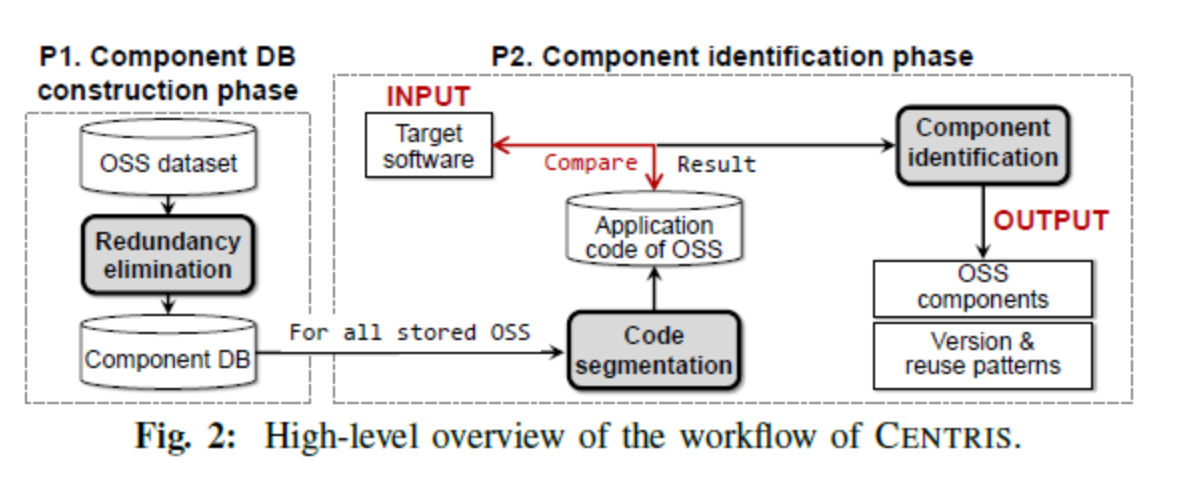
\includegraphics[width=\linewidth]{pics/算法流程.png}
  \caption{算法流程}
\end{figure}
整个流程分为以下两步:
1. 构建数据库
2. 识别目标项目中重用的代码



\subsection{概述}
\begin{figure}[htb]
  \centering
  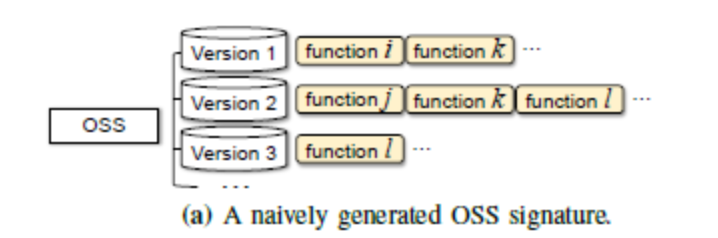
\includegraphics[width=\linewidth]{pics/image-20220622225558096.png}
\end{figure}
上图描述了 CENTRIS 的工作流程。 CENTRIS 包括两个阶段:(1)P1 用于构建 OSS 组件数据库(DB),以及(2)P2 用于识别目标软件中重用的 OSS 组件。 在 P1 中,我们使用了一种称为冗余消除的技术,它可以实现可扩展的组件识别; CENTRIS 通过消除每个 OSS 项目版本之间的冗余来降低组件识别的空间复杂性。 一个 OSS 项目的所有功能都被转换为 OSS 签名,这是一组没有冗余的功能,随后存储在组件数据库中。 在 P2 中,我们使用一种技术,代码分割,来进行精确的组件检测。 具体来说,CENTRIS 通过仅分析 OSS 的应用程序代码在目标软件中重用的模式,最大限度地减少组件检测中的误报。




\subsection{消除冗余}
很多项目在迭代的过程中并不是迭代全部代码的,是在重用上一版代码的基础上进行的更新。直接把各版本的生态组件源代码直接存到数据库中,会造成大量的冗余。

因此我们先需要把这部分的冗余先消除掉。
我们的做法是:
\begin{enumerate}
\item 首先提取训练集中所有版本的C/C++文件
\item 为每个项目创建于版本总数一样多的bin
\item 当同一份代码出现在i个不同版本中时,将这个文件所属的版本信息以及每个版本的路径信息都会存贮在第i个bin中
\end{enumerate}

\begin{figure}[htb]
  \centering
  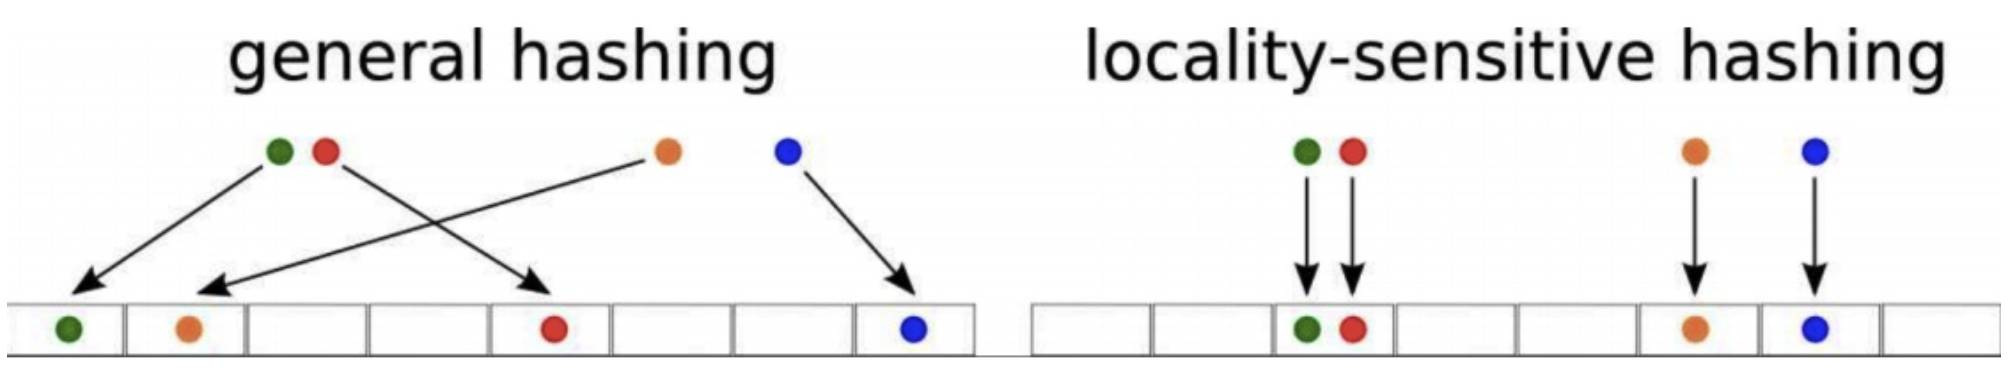
\includegraphics[width=\linewidth]{pics/LSH.png}
\end{figure}

这里我们储存的是C/C++文件的hash值。我们对源代码进行一些处理(删去注释、统一换行与缩进等),然后使用LSH(Locality Sensitive Hash)算法。这样能很好的将代码在高纬空间的相似性映射到低维空间去。

\subsection{重用识别}

对待检测项目的操作:
\begin{enumerate}
    \item 优化组件数据库,保留唯一代码
    \item 从所有检测项目中提取代码
    \item 识别检测项目中的重用组件
\end{enumerate}

假设S为要检查是否包含第三方软件的项目,检测S与我们的组件数据库中的每个项目之间的公共file,如果数据库中存在一个项目P,P与S有一个或多个公共源码文件,则可以确定S和P的关系属于下述四个类别之一。

S和P的关系:

\begin{enumerate}
    \item R1:S和P共享广泛使用的代码
    \item R2: S和P同时重用其他项目
    \item R3:S重用P
    \item R4:P重用S
\end{enumerate}


因为hash算法本身降低了一些精确度,同时一些简单的代码本身存在通用的可能性,所以我们要设定一个阈值来过滤,只有满足以下公式,我们才可以判断为代码重用。


% \begin{theorem}
%   定理内容。
%   “定义”、“假设”、“公理”、“引理”等的排版格式与此相同,详细定理证明、公式可放在附录中。
% \end{theorem}

$\phi(S, P) \geq \theta$

% \begin{proof}
%   证明过程.
% \end{proof}


\subsection{算法分析}
为什么 CENTRIS 是准确的。首先,由于 CENTRIS 在识别阶段不依赖结构信息,因此无论结构变化如何,我们都可以识别组件。接下来,不管OSS是否嵌套,如果每个OSS的应用代码复用率大于θ,就可以识别为正确的组件。最后,CENTRIS 的代码分段不仅可以减少误报,还有助于识别严重修改的组件。考虑开源组件 ArangoDB 的 Velocypack 组件;只有 3.6\% 的 Velocypack 代码库在 ArangoDB 中被重用。事实上,Velocypack 包含了另一个 OSS(GoogleTest),测得 Velocypack 的应用代码重用比例为 12\%。仅突出 OSS 的应用程序代码的重用模式会使目标软件与 OSS 之间的相似度得分在 OSS 是正确组件时更高,而在 OSS 误报时降低(即接近 0\%)。使用这种明显的相似性得分差异,CENTRIS 可以精确识别具有低误报率的修改组件。
\\
\subsubsection{算法优点}

\begin{enumerate}
    \item 识别重用不依赖结构信息,无论结构如何变化都可以识别项目重用的代码
    \item 无论项目是否嵌套,只要代码复用率大于阈值,就可以识别
\end{enumerate}

\subsection{相关工作}
在过去的几十年里,已经提出了许多技术来检测代码克隆CENTRIS采用了基于签名的克隆检测方法。然而,正如我们在本文中所展示的,使用现有的克隆检测技术在识别嵌套 OSS的修改重用时会遭受误报。软件组成分析。现有的 SCA 技术不足以准确识别修改后的 OSS 重用。前人提出了OSSPolice 来查找 Android 应用程序的第三方库。他们利用混淆的恒定特征来提取版本信息并确定是否使用了易受攻击的版本。他们通过分层索引和匹配将误报降至最低。由于他们更关心的是在二进制级别准确识别第三方库,因此,它与我们对检测修改组件的目标不同。但是,商业 SCA 工具,例如 Synopsys Black Duck Hub和 Antepedia的工作没有考虑修改后的重用,因此错过了许多重用的组件。

\subsection{Centris速度优化}
\subsubsection{外存读取}

最初的方法是直接从建成的数据库一条条读取哈希值并且遍历比较,这个方法需要非常多次数的IO交互,速度最慢。
\subsubsection{读入内存}
优化方法是把数据库中哈希值和对应版本号的记录读到内存中,这里是用了一个二维列表hashes[],这样每次的读取都是和内存进行交互,比直接和外存交互快了很多。

\subsubsection{建树}一开始我们想的是把哈希值进行排序,但是后来发现这个方法是完全不可行的,因为这里的tlsh.diff()函数不是直接将哈希值相减得到的,比如两个哈希值第一位不同,那么此时我们对其进行排序的话,,这两个值将隔得很远,但是事实上用diff()函数得到的计算结果会很小,因为他们只差了一位。所以我们必须用一种新的方法,这种方法是真正基于哈希值差距对数据进行组织的:



所以,我们采用了*HAC-T and Fast Search for Similarity in Security* 里面的方法对hash值进行建树,把复杂度从O(n*n)降低到了O(nlogn)。具体方法如下:

快速搜索问题可以看成为一种最近邻搜索: 

我们有一个数据集D,包含项目和相似度或距离度量。 假设距离度量为Dist(d1, d2),对于一个新的数据项S,我们要在其中找到dmin,即D 中最接近S的元素。即D中具有最小Dist(dmin, S) 的元素。

原来论文的方法是逐个比较hash值,直到找到与目标文件hash值相差小于阈值的元素,这个将耗时O(n),大大降低了比较的效率,我们通过建树使其复杂度变成`O(log(n))`。

我们需要避免将S 与D 的所有元素进行比较。理想情况下,我们仅需要将S与D 的一个小子集进行比较,这里我们构建一个搜索树,在其中我们可以在叶节点处存储来自D的多个相似的项目。给定一个新项目,我们可以沿着搜索树追踪一条路径并与最后节点中的项目进行比较。这种方法的一个优点是我们知道查找的计算成本,它与最深树的深度乘以叶子中的项目数成正比,并且复杂度大大降低了。

\subsubsubsection{ BuildTree()}


构建树:首先,我们定义一个 SplitMethod(),如下所示,它具有输入节点 N(我们将 N.data 与 D 的子集相关联) ) 和输出 (Y, T, X1, X2)。 为了使树变得平衡,我们根据各个节点的哈希值和pivot哈希值的差值来把树一分为二,差值较小一半的归为左子树,差值较大另一半的归为右子树。同时我们也定义了叶子节点的大小,如果叶子节点过小,那么分割节点就会比较浪费且没必要。

\begin{figure}[htb]
  \centering
  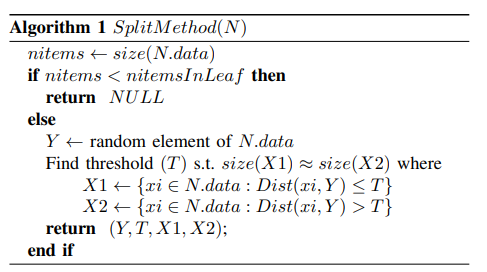
\includegraphics[width=\linewidth]{pics/image-20220622212533508.png}
\end{figure}


然后我们可以通过设置 root.data <- D 并调用 TreeBuild(root) 来构建树:

\begin{figure}[htb]
  \centering
  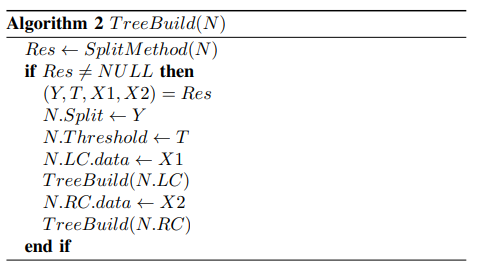
\includegraphics[width=\linewidth]{pics/image-20220622212936887.png}
\end{figure}

\subsubsubsection{SearchTree()}

我们可以通过执行 Search(root, S) 在树中搜索项目 S 的项目,该搜索函数返回离 S 最近的项目.

\begin{figure}[htb]
  \centering
  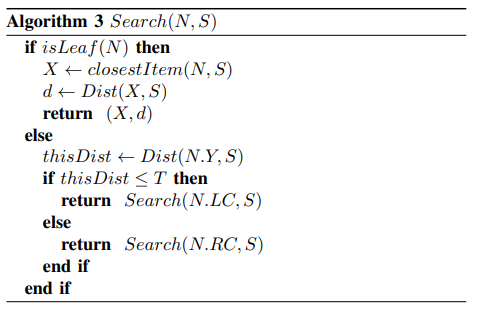
\includegraphics[width=\linewidth]{pics/image-20220622213044543.png}
\end{figure}


在本项目的实现中,为了结果更加直观,还向用户提供了accuracy参数,因为建树搜索是一个近似算法,而且叶子节点的大小决定了算法的精确度,叶子节点越小,精确度越高,但是复杂度也会越高,通过调整accuracy参数,我们可以控制叶子节点的大小来调整代码克隆检测的精确度和复杂度。


\section{结果分析与比较}

\subsection{水平比较:Centris和 SourceCC}


可见,SourceCC的准确度高于Centris。

而对于大数据集来说,SourceCC由于复杂度较高且受限于硬件条件,无法跑,而Centris可以轻松完成比较,因为Centris的搜索复杂度低于SourceCC。





\subsection{ 垂直比较:Centris的不同搜索比较方法,不同大小的数据集检测结果}
\subsubsection{ 不同搜索方法}
首先我们用一个比较小的训练集进行测试,训练集包含了49个glibc的版本。
\subsubsubsection{ 外存比较}
\begin{figure}[htb]
  \centering
  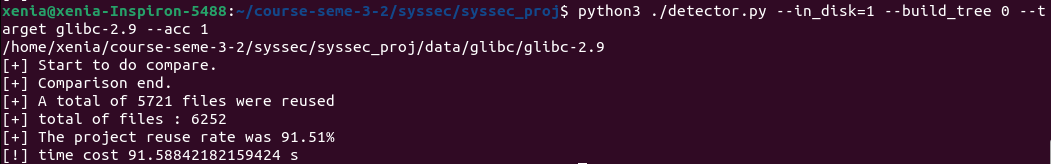
\includegraphics[width=\linewidth]{pics/image-20220622221558771.png}
\end{figure}

   这里用了91s+。

\subsubsubsection{ 内存比较}

\begin{figure}[htb]
  \centering
  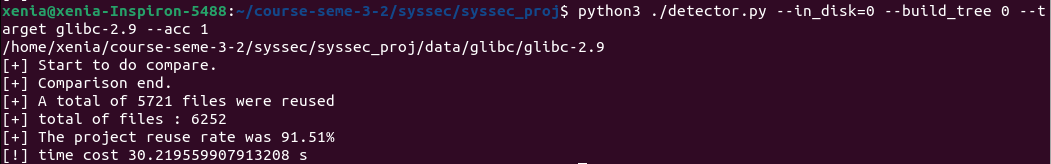
\includegraphics[width=\linewidth]{pics/image-20220622221549800.png}
\end{figure}

   这里用时30s+。

\subsubsubsection{ 建树比较}
\begin{figure}[htb]
  \centering
  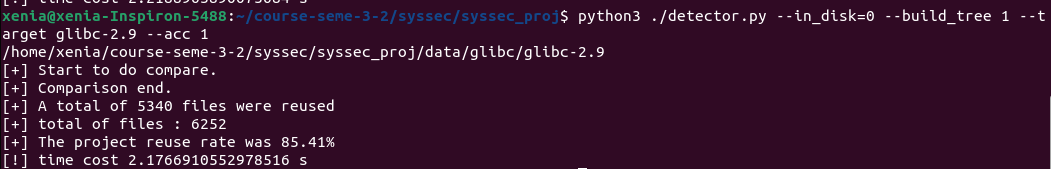
\includegraphics[width=\linewidth]{pics/image-20220622221526098.png}
\end{figure}

   这里用时2s+。

   

\subsubsection{ 不同大小的数据集}
\subsubsubsection{ 很小数据集 minisql
}
   

\subsubsubsection{ 较小数据集 glibc}
   
\subsubsubsection{大数据集 }










% \begin{procedure}
%   \caption{过程名称}
%   \small
%   \begin{algorithmic}
%     \REQUIRE
%     \ENSURE
%     \STATE \COMMENT{《计算机学报》的方法过程描述字体为小5号宋体,IF 、THEN等伪代码关键词全部用大写字母,变量和函数名称用斜体}
%   \end{algorithmic}
% \end{procedure}

% \begin{algorithm}
%   \caption{算法名称}
%   \small
%   \begin{algorithmic}
%     \REQUIRE $n \geq 0 \vee x \neq 0$
%     \ENSURE $y = x^n$
%     \STATE $y \leftarrow 1$
%     \IF{$n < 0$}
%       \STATE $X \leftarrow 1 / x$
%       \STATE $N \leftarrow -n$
%     \ELSE
%       \STATE $X \leftarrow x$
%       \STATE $N \leftarrow n$
%     \ENDIF
%     \WHILE{$N \neq 0$}
%       \IF{$N$ is even}
%         \STATE $X \leftarrow X \times X$
%         \STATE $N \leftarrow N / 2$
%       \ELSE[$N$ is odd]
%         \STATE $y \leftarrow y \times X$
%         \STATE $N \leftarrow N - 1$
%       \ENDIF
%     \ENDWHILE
%   \end{algorithmic}
% \end{algorithm}



% \begin{acknowledgments}
%   致谢内容。
% \end{acknowledgments}


\nocite{*}

\bibliographystyle{cjc}
\bibliography{example}


\newpage

% \appendix

% \section{}

% 附录内容置于此处,字体为小5号宋体。附录内容包括:详细的定理证明、公式推导、原始数据等


\makebiographies


\begin{background}
*论文背景介绍为英文,字体为小5号Times New Roman体*

论文后面为400单词左右的英文背景介绍。介绍的内容包括:

本文研究的问题属于哪一个领域的什么问题。该类问题目前国际上解决到什么程度。

本文将问题解决到什么程度。

课题所属的项目。

项目的意义。

本研究群体以往在这个方向上的研究成果。

本文的成果是解决大课题中的哪一部分,如果涉及863/973以及其项目、基金、研究计划,注意这些项目的英文名称应书写正确。
\end{background}

\end{document}
